% !TEX root = ../main.tex

% 第一章一般名为绪论/引言,不可省略

\chapter{绪论}

\section{研究背景}
随着计算机图形学、计算机辅助设计和多媒体技术的发展,三维模型越来越多地应用于人们的生产和生活中,并成为人们生活中不可或缺的一部分。三维模型被广泛应用于计算机游戏、电影和其他虚拟现实的应用中,通过对三维模型的渲染,人们可以看到逼真的图像,获得美妙的视觉体验。随着虚拟现实技术的兴起,三维模型也成为了一个越来越重要的角色。三维模型被广泛应用与工业制造,现在很多产品在批量生产之前,都会先通过计算机辅助设计软件在计算机中生成三维模型。新兴的3D打印技术更是让这个过程变得更加便捷,让我们可以将大多数三维模型变成现实的物品。
在计算机中,三维模型主要表示方式有两类:连续的表示方法和离散的表示方法。连续的表示方法如代数曲面可以很精确并以很少的数据量来表示一个简单模型的表面,但是对于很多模型很难找到一个曲面的解析表达。因此,在计算机中我们常用离散的三角形或多边形网格来表示一个三维模型,其中我们最常的是三角形网格表示法。
现在三维模型的主要来源有两个:(1)依靠计算机辅助设计,人工制造;(2)依靠三维扫描仪扫描之后重建得到。得益于三维扫描仪,三维模型种类和数量大增。现在三维模型不仅复杂度日益增加,而且对三维模型的细节和精度的要求也日益提高,更丰富的细节和更高的精度在使得基于三维模型的计算机应用带给我们更多的真实感,使得工业制造更加精准的同时,也使得三维模型数据量大增,使得对三维模型的存储、传输、显示、修改这些基本操做带来了相当大的困难,而且使得很多计算机图形学的算法的计算量也大幅度增加。而对于一般的应用需求,在很多时候并不需要高精度的细致的三维模型,因此在一个较低的误差范围内,用一个顶点(或三角面片)数量尽可能少的三角网格来近似原网格成为了一个迫切的需求。

%% 绪论第一节一般是研究背景,
%% 交待下这个领域遇到了什么亟待改善的困境。
%% 从严谨的学术观念考虑,必须引用足量的数据描述现状,
%% 避免使用过多主观判断的语句和用词。

\section{相关工作}

网格简化算法的研究已经有一段时间了,在相关网格简化算法之中常用的三角网格简化操作有消点,顶点聚簇合并,消边等。顶点的消点操作是指在消除一个三角形网格上的一个顶点以及包含该顶点的边和面形成一个洞,然后利用该洞的边界点的组合构成的三角形补洞(如图\ref{fig:rm-vertex})。顶点聚簇合并是指通过同时合并两个或多个三角网格上的顶点的方式来减少顶点和三角面片(如图\ref{fig:clu-vertex})。消除边操作可以看做是顶点聚簇合并的一个特例,要求一次只能合并构成一条边的两个顶点。
\begin{figure}[htbp]
    \centering
    \includegraphics[width=.8\textwidth]{vertex_remove.png}
    \caption[顶点删除]{通过顶点删除的操作简化网格,图来自\cite{mesh-simp}}
    \label{fig:rm-vertex}
\end{figure}
\begin{figure}[htbp]
    \centering
    \includegraphics[width=.8\textwidth]{vertex_clustering.png}
    \caption[顶点聚簇合并]{通过顶点聚簇合并的操作简化网格,图来自\cite{mesh-simp}}
    \label{fig:clu-vertex}
\end{figure}
在网格简化算法中,我们通常用Hausdorff距离\cite{hausdorff-dis}被用来作为衡量简化结果与原网格之间的误差。单个
点$x\in\mathbb{R}^3$到一个三角网格$F$的 Hausdorff 距离定义为:
\begin{equation}
  d(x, F) = \underset{y\in F}{inf}||x-y||
  \label{eq:v2f-haus}
\end{equation}
这里y是三角网格F表面上的任意一点,inf表示取最小值。定义三角网格$F_1 \to F_2$的最大Hausdorff距离为:
\begin{equation}
  \rho_{max}(F_1,F_2)=\underset{x\in F_1}{sup}(x,F_2)
  \label{eq:f2f-max-haus}
\end{equation}
这里sup表示取最大值。定义三角网格$F_1 \to F_2$的平均Hausdorff距离为:
\begin{equation}
  \rho_{mean}(F_1,F_2)=\underset{x\in F_1}{avg}(x,F_2)
  \label{eq:f2f-mean-haus}
\end{equation}
这里avg表示取平均值。定义三角网格$F_1 \to F_2$的Hausdorff距离的均方根(RMS)为:
\begin{equation}
  \rho_{rms}(F_1,F_2)=\underset{x\in F_1}{rms}(x,F_2)
  \label{eq:f2f-rms-haus}
\end{equation}
定义两个三角网格之间的双向最大Hausdorff距离和双向平均Hausdorff距离以及双向Hausdorff 距离的均方根分别为:
\begin{equation}
  \begin{array}{l}
    d_{H\_max}(F_1,F_2)=sup(\rho_{max}(F_1,F_2), \rho_{max}(F_2,F_1))\\
    d_{H\_mean}(F_1,F_2)=sup(\rho_{mean}(F_1,F_2), \rho_{mean}(F_2,F_1))\\
    d_{H\_rms}(F_1,F_2)=sup(\rho_{rms}(F_1,F_2), \rho_{rms}(F_2,F_1))
  \end{array}
  \label{eq:ff-haus}
\end{equation}
相同的Hausdorff距离下,比较网格的简化程度(顶点或三角面片数量),或者相同的简化程度下比较简化之后的网格和原网格之间的Hausdorff距离是比较两个网格简化算法的重要依据。根据给定不同的网格简化条件,当前的简化算法可以分为两类:$Min−\#$类算法和$Min−\varepsilon$类算法\cite{simp-envlop}。$Min−\#$类算法给定一个误差范围ε以及其计算方式,在保证简化的结果与原模型间的误差不允许超过ε的条件下做网格简化。$Min−\varepsilon$类算法则在给定一个最终的简化结果的顶点或三角面片数量的条件下,尽可能地最小化简化结果与原网格之间的误差。\par

在所有$Min−\varepsilon$类简化算法中,Michael Garland等人提出的QEM算法\cite{qem1}具有简单高效的特点,是主流的网格简化算法之一。现在,我们可以下载到实现该算法的开源应用QSlim。其主要思想是在做顶点合并时,最优化(最小化)每个顶点到其所属平面集合的距离平方和,从而将降低每次简化带来的误差。在QEM算法中,每一个模型被视为是由很多个离散的有限平面所组成,而模型上的每一个顶点就是其一环邻域(周围的一圈)平面的交点。因此,我们将顶点$v=[x,y,z,1]^T$和一系列平面关联起来,相当于每一个顶点$v$都应该在一个平面集合$\text{planes}(v)$的每个平面上。每一个$\text{plane}(v)$都可以表示为$p^Tv=0,p=[a,b,c,d]^T,a^2+b^2+c^2=0即ax+by+cz+d=0$,从而该顶点到这个平面$\text{plane}(v)$的距离的平方可表示为$(p^Tv)^2$即$v^Tpp^Tv$,每一个顶点到其平面集合的距离平方和为
\begin{equation}
  \Delta(v) = \sum_{p\in \text{planes}(v)}v^Tpp^T = v^TQ_vv
\end{equation}
我们称$\Delta(v)$为Quadric Error在初始的情况下$\forall v,\Delta(v)=0$。在QEM算法中,我们用这个Quadric
Error作为简化结果与原模型的距离衡量标准。当我每做一次顶点合并$(v_0, v_1) \to v̅$时,我们将这两个顶点的平面集合合并成为新的顶点的平面集合即planes(v̅) = planes(v 0 ) ∪ planes(v 1 ),从而会产生一个新的Quadric Error:$\Delta(v̅)=v^T(Qv_0+Qv_1)v$。该算法以最小化Quadric Error的上界为目标,每次都是以贪心的策略从可合并的顶点对(构成一条边的两个顶点,或者两个距离小于一定阈值的顶点)中选取$\Delta(v̅)$最小的顶点对做合并。该算法实现起来非常简单,可以归纳为以下几步:
\begin{enumerate}[(1)]
  \item 初始化每个三角网格上的顶点的矩阵Q;
  \item 通过$\text{minimize} \; v̅^T(Qv_0+Qv_1)v̅$,计算每一条边的两个顶点的最优合并点$v̅$ ,以$\Delta(v̅)$作为这条边合并的代价,以此一个最小优先级队列;
  \item 迭代地从最小优先级队列中取出一个顶点对进行合并,然后更新这个优先级队列。
\end{enumerate}
QEM方法不仅简单高效,在大程度的简化要求下,简化结果也能非常好地保持原模型的视觉效果(如图\ref{fig:qem-res})。
\begin{figure}[htbp]
    \centering
    \includegraphics[width=.7\textwidth]{qem_res.png}
    \caption[QEM算法结果]{使用QEM算法将模型budda从1,085,634个面(a),简化到20,000个面(b-c)和1,000个面(d-e),图来自\cite{qem2}}
    \label{fig:qem-res}
\end{figure}

与该算法相似的还有Peter Lindstrom等人提出的Memoryless Simplification网格简化算法\cite{memory-less},也是通过贪心的策略迭代地合并顶点。与前者不同的是该算法将$(v_0,v_1) \to \bar{v}$的Quadric Error定义为网格简化时由于顶点合并所带来的与上一步的结果之间构成的体积即:
\begin{equation}
  \Delta_1(\bar{v}) = \sum_{t_i \in \text{one\_ring}(v_0) \cup \text{one\_ring}(v_1)} \text{det} (\bar{v},v_0^{t_i},v_1^{t_i},v_2^{t_i})^2
\end{equation}
这里$t_i$是顶点$v_0$或顶点$v_1$一环邻域的三角形,$v_0^i,v_1^i, v_2^i$是这个三角形$t_i$上的三个顶点(如图\ref{fig:memory-less})。该算法相当于在标准Quadric Error的基础上,将每个平面的面积作为一个权重加入到了Quadric Error的计算中去。与此同时,当存在多对顶点的Quadric Error相同时加入了尽量保持网格质量(三角形每条边尽可能相等,不出现细长三角形)的约束,让$\bar{v}$所构成的边的平方和最小,即:
\begin{equation}
  \Delta_2(\bar{v}) = \sum_{v_i \in \text{one\_ring} (v_0,v_1)} (\bar{v}-v_i)^2
\end{equation}
\begin{figure}[htbp]
    \centering
    \includegraphics[width=.7\textwidth]{memory_less.png}
    \caption[顶点合并操作]{顶点合并操作示意图,边e被合并到顶点v,三角形$t_7$和$t_8$在合并的过程中被删除。第二行的三个四面体显示了合并时由三角形$t_0,t_3,t_8$与合并顶点$v$所构成的体积,图来自\cite{memory-less}}
    \label{fig:memory-less}
\end{figure}
该算法通过这种保体积的策略,能得到比QEM算法更优的简化效果。由于在确定一个定点对的合并点位置时,需根据体积优化顶点位置,因此需要消耗的时间是QEM的10倍左右。此外,该算法和QEM算法的一个很大的不同点是此方法的Quadric Error以上一次的迭代结果为计算标准,而标准的QEM的Quadric Error以初始化的网格为计算标准。因此,在相同条件下此方法通过一步步的优化迭代,该算法的结果的平均误差(平均Hausdorff距离——\ref{eq:f2f-mean-haus})优于很多其他常用的网格简化算法,但在最大误差上逊于其他常用网格简化算法(如图\ref{fig:memory-less-compare})。
\begin{figure}[htbp]
  \centering
  \begin{subfigure}[b]{0.7\textwidth}
    \includegraphics[width=\textwidth]{memory_less_mean_compare.png}
    \caption[input]{平均Hausdorff距离的比较}
    \end{subfigure}
    \begin{subfigure}[b]{0.7\textwidth}
      \includegraphics[width=\textwidth]{memory_less_max_compare.png}
      \caption[mls]{最大Hausdorff距离的比较}
    \end{subfigure}
    \caption[Memory Less简化结果]{Memory Less算法在horse模型上和其他算法的简化结果的比较,图来自\cite{memory-less}}
    \label{fig:memory-less-compare}
\end{figure}

为了满足在高精度范围内简化网格的需求,产生了$Min−\#$类算法,其中最具代表性的算法之一是Jonathan Cohen等人提出的一种基于内外壳的网格简化算法\cite{simp-envlop}。在用户给定最大误差$\varepsilon$的条件下,该算法首先生成与原始网格距离为$\varepsilon$的内外壳边界,然后在保证新生成的三角面片不与内外壳相交的条件下做顶点合并。该算法主要分为三步:
\begin{enumerate}[(1)]
  \item 根据用户给定的误差$\varepsilon$,构建内外壳;
  \item 遍历并尝试删除每一个顶;
  \item 测试补洞后的网格是否在壳内,从而决定是否接受这次简化。
\end{enumerate}
\par 为了保护原模型的拓扑结构,在构建内外壳时,我们需要保证内外壳既不能相交,也不能自交。为了做到这点,Jonathan Cohen等人提出了两种方案:基于分析的构建方法和基于数值的构建方法。在基于分析的构建方法(如图\ref{fig:compute-envlop0}),先为原网格的每一个三角形$t_i$,沿着每个顶点的法向构建一个上下分别$2\varepsilon$厚的棱柱$t_{p_i}$。然后判断每个棱柱$t_{p_i}$上的两个三角面片$\Delta_i$是否与其他棱柱相交,若与某一个棱柱$t_{p_j}$相交,则计算出在三角形$\Delta_i$上并处于棱柱$t_{p_j}$内,离三角形$t_j$的最近点的距离$\delta_{ij}$。做完所有这样的计算后,将对每一个三角形$t_i$的厚度设置为所有$\delta_{ij}$的最小值,即$\epsilon(t_i) = \text{min} \; \delta_{ij}$,而真正构建内外壳每个顶点沿法向移动的距离为$\epsilon(v) = \text{min} \; \epsilon(t_i),t_i \in \text{one\_ring}(v)$。而基于数值的构建方法,在刚开始时内外壳和原模型重合,给定一个沿法向移动的步长k,逐步地移动内外壳顶点直到达到给定的误差ε或者是检测到某三角形与其他非邻接三角形相交。为了得到一个更大的内外壳,在检测到相交并放弃移动内外壳一顶点时,将该顶点的步长设置为原来的$\frac{1}{2}$,继续尝试,直到该步长小于一定阈值之后再停止。当然对于每一个顶点可以选择不同的步长初始化,比如选取其一环邻域中对短的边的边长。\par
\begin{figure}[htbp]
    \centering
    \includegraphics[width=.7\textwidth]{compute_envlop_0.png}
    \caption[分析建壳方法]{基于分析的建壳方法示意图,图来自\cite{simp-envlop}}
    \label{fig:compute-envlop0}
\end{figure}
构建了内外壳之后,通过删除顶点的方式简化网格。一种简单的方式是:把每个顶点放入删除队列,然后依次送队列中取出一个顶点,尝试删除这个顶点以及其一环邻域的所有三角形,从而在原模型上产生一个洞。然后在不添加顶点的情况下,通过添加由边界点构成的三角形来补洞(有多种组合)。测试是否存在一种组合不与内外壳相交,若存在,则接受这个简化并将其邻接的顶点重新加入到队列中;若不存在,则放弃这次简化,模型保持不变。相对于尝试所有可能的补洞组合,另外一种高效的贪心补洞算法是:选取一个满足约束条件(不与内外壳相交)的三角形补上,然后递归地补上由于补上该三角形之后所产生的小的三个(或更少)的三角形。如果这种递归的补洞方法失败,则认为这个顶点删除失败即不能在保证误差的前提下通过删除这个顶点来简化网格。\par
该算法的优点是,能保证双向的Hausdorff距离在给定的误差范围内,真正做到了简化结果与原来网格之间的误差控制。而该算法的缺点也显而易见:(1)受限于内外壳不能相交这个条件,真正的$\varepsilon$不会太大,因此不能对模型做大程度的简化;(2)需要不断地做三角面片的相交检测,因此非常耗时。


而在同样给定最大误差$\varepsilon$的条件下,Borouchaki等人提出了一种能够直接约束Hausdorff距离不超过$\varepsilon$的网格简化算法——MMGS\cite{mmgs},在MMGS中还通过翻面和顶点光顺优化了顶点的位置。
该算法的主要思想是,在用户给定误差精度$\varepsilon$的条件下,通过消边的方式做网格简化,在此过程中通过直接计算简化结果和原网格之间的Hausdorff距离,从而保证误差在$\varepsilon$内,另外,通过加入法向的约束使得简化结果更加光滑,该算法还将在处理的过程中加入了翻边和顶点移动这些网格优化算法,简化和优化迭代进行。\par
对于模型法向的控制,与QEM算法的简化模型中法向基本一致的光滑区域的想法类似但也有所不同的是,该算法要求消除一条边PQ(将P合并到Q如图\ref{fig:mmgs-normal-cond})之后,新生成的任意一个三角形K′的与其周围的三角形法向基本一致也即简化之后的模型尽可能光滑,K需满足:
\begin{equation}
  \forall K, \quad \langle v_k (K), v(K) \rangle \ge cos(\theta)
\end{equation}
\begin{figure}[htbp]
    \centering
    \includegraphics[width=0.7\textwidth]{mmgs_normal_cond.png}
    \caption[法向约束]{法向约束示意图,图来自\cite{mmgs}}
    \label{fig:mmgs-normal-cond}
\end{figure}
这里$v_k(K)$是顶点v上的法向,$v(K)$是三角形K上的法向,$\langle ..,.. \rangle$表示点积,而$\theta$则是用户给定的一个阈值。\par
对于Hausdorff距离的控制该算法保证新生成的三角形$K'$与原模型之间的Hausdorff距离小于$\varepsilon$,即$d_H(K',T^{ref})\le\varepsilon$,也就是说需要保证$d_H(K',\mathcal{R}(p))+d_H(\mathcal{R}(P),T^{ref}) \le \varepsilon$这里$\mathcal{R}(P)$是顶点P的一环邻域的三角形,$T^{ref}$表示原网格。对于$d_H(K',\mathcal{R}(P))$,即图中两块蓝色区域的Hausdorff距离,这可以通过简化前后拥有相同边(如图\ref{fig:mmgs-calc-haus}中红色的边)的三角形$\widetilde{K},K$之间的Hausdorff距离的最大值来近似,即
\begin{equation}
  d_H(K', \mathcal{R}(P)) \approx \text{max} \; d_H(K',\widetilde{K})
\end{equation}
\begin{figure}[htbp]
  \centering
  \begin{subfigure}[b]{0.4\textwidth}
    \includegraphics[width=\textwidth]{mmsg_hausdorff_calc_0.png}
    \caption[input]{简化前}
    \end{subfigure}
    \begin{subfigure}[b]{0.4\textwidth}
      \includegraphics[width=\textwidth]{mmsg_hausdorff_calc_1.png}
      \caption[mls]{简化后}
    \end{subfigure}
    \caption[MMGS计算Hausdorff距离]{计算Hausdorff距离示意图}
    \label{fig:mmgs-calc-haus}
\end{figure}
因此,对于每个新的生成的三角形$K'$,需要满足的Hausdorff距离条件又可以表示为:
\begin{equation}
  d_H(K',\mathcal{R}(P))+\underset{K\in\mathcal{R}(P)}{\text{max}}\;h(K) \le \varepsilon
\end{equation}
这里$h(K)$表示三角形K到原网格的Hausdorff距离的最大值。\par
除了在给定的Hausdorff距离内简化模型之外,与其他算法相比,在整个过程中通过翻边和移动顶点等模型优化算法,使得简化结果更加光滑(美观)如图\ref{fig:mmgs-res}。当然作为补偿,该算法相对其他简化算法有着更大的平均Hausdorff距离。同事我们可以看到,该算法是很多算法的综合体,因此复杂程度高,实现难度大,不过幸运的是我们可以在开源软件OpenFlipper中找到实现该算法的源代码。
总的来说,该算法主要分为以下几个步骤:
\begin{enumerate}[(1)]
  \item 在满足误差和法向的约束的前提下消边
  \item 通过翻边和移动顶点优化网格
\end{enumerate}
\begin{figure}[htbp]
  \centering
  \begin{subfigure}[b]{0.4\textwidth}
    \includegraphics[width=\textwidth]{mmgs_res_0.png}
    \caption[input]{简化前}
    \end{subfigure}
    \begin{subfigure}[b]{0.4\textwidth}
      \includegraphics[width=\textwidth]{mmgs_res_1.png}
      \caption[mls]{简化后}
    \end{subfigure}
    \caption[MMGS简化结果]{MMGS的简化结果示意图,引用自\cite{mmgs}}
    \label{fig:mmgs-res}
\end{figure}

在2015的SIG上Manish Mandad等人发表了一种将网格重建和基于内外壳简化算法相结合的网格近似算法\cite{isotopic-appro},该算法也是本文主要参考的算法。该算法能在给定内外边界采样点的情况下,先通过细化,重建出一个误差空间的近似,在此基础上通过消边来简化这个四面体结构,从而生成一个尽可能简化的网格去近似原网格,该算法我们将在下一章详细介绍。

各向异性网格的生成是一个被广泛研究的问题。在最近二十年内,许多基于Delaunay三角化技术的各向异性网格生成技术被提出。在各向同性的Delaunay三角化中,网格顶点的插入依赖于所谓的Delaunay核。\cite{Frey:2007:MGA:1205626, Dobrzynski2008}介绍的各向异性网格生成方法通过扩展传统的Delaunay核来实现各向异性顶点的插入, 从而满足指定的各向异性度量要求。 Boissonnat\cite{Boissonnat:2008:LUA:1377676.1377724, boissonnat:inria-00615486, boissonnat:hal-01146307}提出了一种基于受约束星形集合的ADT技术。 该方法通过基于受约束星形集合的Delaunay细化来实现各向异性的Delaunay三角化。 当度量场和定义域的边界是平滑时, 该方法可以得到较高质量的网格。 但该方法的效率较低, 而且只能处理比较平滑的度量场, 即各向异性比例在定义域中变化较为缓慢的情形, 因此并不实用。

另一类方法通过扩展基于Voronoi图的Delaunay三角化方法来生成各向异性网格。 这类方法通过顶点插入扩展传统的Voronoi图来实现为各向异性的Voronoi图(AVD)实现各向异性的Delaunay三角化。 \cite{Labelle:2003:AVD:777792.777822}通过顶点插入来优化得到AVD, \cite{Du:2005:ACV:1046640.1046658, Valette:2008:GRT:1340081.1340168, Levy:2010:LPC:1778765.1778856, bruno:hal-00804558}则通过优化各向异性中心Voronoi细分(AVCT)能量函数得到AVD。 以上几种方法迭代优化AVD的效率较低, 而且不能保证优化得到的AVD对偶的ADT是一个流形网格\cite{Canas2011}。 还有一种构造AVD的方法是基于粒子之间的相互作用力\cite{ATPSCPE, PASM}。 这种方法通过优化粒子的位置使得粒子达到平衡状态, 然后计算这些粒子的AVD。 基于粒子的方法最主要的优点是与网格无关, 其缺点是当各向异性比例变化剧烈时, 核函数的宽度等参数的选择对结果质量的影响很大。同样地, 基于粒子的方法也不能保证优化得到的AVD对偶的ADT是一个流形网格。
基于Delaunay三角化的各向异性网格自适应技术也是一类常见的各向异性网格生成技术\cite{Jiao2009}。 这类方法的主要思想是在Delaunay网格上进行局部的网格修改操作, 从而实现各向异性的自适应。然而这种自适应的方法不适用于固定顶点的各向异性三角化。

\section{本文工作}
通常我们以以下几个方面来评价一个网格简化算法:
\begin{enumerate}[(1)]
\item 相同误差下简化程度的高低和相同顶点数量下简化误差的大小;
\item 能否较好地保持原网格的法向信息;
\item 算法是否高效简单。
\end{enumerate}

%% 现在的一些主流的方法,虽然能够较好地满足一般用户的需求。但是均无法做到能够鲁棒地处理各种输入数据的同时能够严格地控制简化误差。而最近 Manish Mandad等人提出的保拓扑的网格近似算法\cite{isotopic-appro},很好地做到了前三点。我们在实现其算法的基础上,对其可能存在的不足做了分析,并实现了我们的改进。Manish Mandad等人提出的保拓扑的网格近似算法大致可以分为以下几个步:细化、简化误差边界、镶嵌0-等值点、简化0-等值面和消除所有可能消除的边。该算法以在误差空间Ω的内外边界(内外壳)上密集的采样点S来作为输入数据,在细化阶段,以这些采样点的包围球的3D Delaunay三角化作为初始化,在这个三角化的每个四面体上维护一个线性差值函数,其中包围球和外壳采样点的值定为1,内壳采样点的值定为-1。然后不断地往这个三角化中加入内外边界的采样点,直到这个差值的0-等值面(所有差值为0的点构成的面)能够将所有的内外采样点区分开,这样就得到了一个原误差空间的近似$\Gamma$。简化误差边界,就是在保持0-等值面仍能够区分内外采样点的条件下去尝试消除误差空间Γ边界上的边。镶嵌0-等值点,则是将所有在边上的0-等值点插入到这个三角化中。在镶嵌0-等值点之后,就得到了显式的0-等值面——原网格的一个近似,不过这0-等值面还不够简化,需要在保持0-等值面任然能够将内外采样点区分开的条件下,可以去尝试消除每一条由0-等值点所构成的边。之后为了进一步简化,再同样条件下,继续消除所有可能消除的边。由于该算法始终确保0-等值面能将内外采样点分开这个条件,因此能够严格地控制误差。由于在整个简化过程中依次遍历所有可能消除的边,在消边时则通过对附近空间采样去寻找可能的合并点的位置,因此,在简化结果上,与以往的算法比较具有明显优势。

现在的一些主流的方法,虽然能够较好地满足一般用户的需求。但是均无法做到能够鲁棒地处理各种输入数据的同时能够严格地控制简化误差。而最近 Manish Mandad等人提出的保拓扑的网格近似算法\cite{isotopic-appro},该算法以在误差空间Ω的内外边界(内外壳)上密集的采样点S来作为输入数据,通过以下几个步骤:细化、简化误差边界、镶嵌0-等值点、简化0-等值面和消除所有可能消除的边,来达到简化网格的目的。在简化过程中始终确保0-等值面能将内外采样点分开这个条件,因此能够严格地控制误差。在简化结果上,与以往的算法比较具有明显优势。我们在该算法的基础上,对其可能存在的不足做了分析,提出了我们的改进策略。

在这个保拓扑的网格近似算法的细化阶段,使用了3D Delaunay三角化来构建四面体网格结构,虽然这样能够拥有较好地质量,但并没有考虑到原三角网格本身存在的各向异性,从而使得接下来需要经过消边来获得这个特性。我们提出,可以通过一个各向异性的3D Delaunay三角化,来替代原有的各向同性的3D Delaunay三角化,从而获得一个更好的初始化结果,并优化最终简化结果。我们通过根据原三角网格上的曲率信息构建一个能够体现其各向异性信息的黎曼度量,通过能量优化将该各向异性的黎曼度量转化为各向同性的黎曼度量,在各向同性的黎曼度量下做3D Delaunay三角化,从而得到一个在原空间中各向异性的3D Delaunay三角化。实验证明这样的初始化,不仅大大简化了细化的结果——得到了一个更好的初始化状态,而且优化了最终结果——在给定的误差范围内,进一步减少了最终简化结果的顶点数量。

\section{论文的内容和结构安排}
首先我们介绍了现阶段三角网格简化在计算机图形学和计算机辅助设计中的重要意义,以及现阶段三角网格模型简化的背景,并介绍了现在国内外的一些研究成果和算法以及它们各自的优势和不足。然后提出了我们认为的三角网格简化的几个目标,并着重介绍了Manish Manad等人的保拓扑的网格近似算法,然后介绍了我们改进的基于Manish Manad等人的算法的改进及其具体实现。最后是我们对三角网格简化工作的总结和展望。\par
本文的章节安排如下,第一章介绍网格简化的背景和国内外对网格简化的研究现状,以及本文的主要工作;第二章,详细描述了Manish Mandad等人提出的基于内外壳的网格近似算法;第三章,我们基于Manish Mand提出的算法的改进和算法的实现;第四章,我们的算法的实现以及结果展示;第六章是总结和展望。
